%Kelompok BSD
%Dwi Yulianingsih
%Arjun Yuda Firwanda
%Dwi Septiani Tsaniyah
%Jeremia Wahyudi Sianturi
%Ervanda Rambu Anarky

\section {Bit Byte}
Bit dan Byte memiliki arti istilah yang sering kita dengar atau temukan ketika berurusan dengan komputer atau internet.Sebutan yang seperti ini sering sekali biasanya dapat membuat kita menjadi bingung dan linglung. Bit merupakan kependekan dari istilah “Binary Digit” yang memiliki arti digit bener.
Binary digit adalah satuan-satuan terkecil dalam komputasi digital. Komputer tidak menggunakan angka desimal  dalam menyimpan data nya. Semua data komputer yang sudah ada akan disimpan dalam sebuah angka – angka biner. Dan hanya dua nilai yang bisa dinyatakan 1 bit, yaitu 0 maupun nilai 1, dalam telekuminkasi digital juga seperti itu, semua level tegangan diubah menjadi bentuk data biner.
Sedangkan byte adalah satuan informasi dalam computer yang lebih besar dari bit. Istilah “Byte” pertama diciptakan oleh Dr. Werner Buccholz di tahun 1956, saat itu ia bekerja sebagai seorang ilmuan di IBM. 
Cara membedakan bit dengan Byte adalah dengan mengingat bahwa  huruf “b” kecil untuk bit yang artinya lebih kecil dari Byte, sedangkan “B” besar untuk Byte arinya niainyalebih besar dari bit.
di dalam media penyimpanan itu seperti hardisk,flashdisk, compack disk (CD) atau memory card, kita semua mengenal istilah atau satuan untuk menyebutkan ukuran atau kapasitas dari media penyimpanan, seperti kilo byte, mega byte, giga byte dan tera byte. Dan jika kita ingin mengetahui sebuah informasi suatu ukuran file ( document, photo, video, dan lain-lain
Hardisk maupun flashdisk biasanya akan dimunculkan dalam sebuah satuan Kilo Byte (KB), Mega Byte (MB), Giga Byte (GB), TeraByte (TB), Bytes ataupun yang terkecil dimunculkan dalam satuan Bit. Biasanya untuk file – file yang berukuran kecil atau kurang dari satu Mega Byte (1MB) akan ditampilkan dalam satuan Kilo Byte (KB).
dalam \cite{tucker2012bit} dikatakan bahwa ada 12 macam satuan dalam Byte, yang diantaranya adalah :

\begin{figure}[ht]
\centerline{\includegraphics[width=1\textwidth]{figures/lihatlah.png}}
\caption{gambar lihatlah.}
\label{lihatlah}
\end{figure}
\ref{lihatlah}
contoh gambar

1 Bit = BinaryDigit
8 Bit = 1 Byte
1024 Bytes = 1 KiloByte (KB)
1024 Kilo Bytes = 1 MegaByte (MB)
1024 Mega Bytes = 1 GigaByte (GB)
1024 Giga Bytes = 1 TeraByte (TB)
1024 Tera Bytes = 1 PetaByte (PB)
1024 Peta Bytes = 1 ExaByte (EB)
1024 Exa Bytes = 1 ZettaByte (ZT)
1024 Zetta Bytes = 1 YottaByte (YT)
1024 Yotta Bytes = 1 BrontoByte (BB)
1024 Bronto Byte= 1 GeoByte

Pada artikel ini kami akan membahas 4 satuan yang diantaranya adalah Kilo Byte (KB), Mega Byte (MB), Giga Bytes (GB), Tera Bytes (TB), Peta Byte (PB) dan cara untuk mengkonversikannya. Contoh dari Kilo ke Mega atau dari Mega ke Giga. 
Sebelum itu mari kita bulatkan angka 1024 menjadi 1000 agar lebih mudah dikonversi. \cite{menon1999nanotechnology}
contoh gambar untuk mengkonversi 
\ref{Bytes.JPG}
contoh gambar

\begin{figure}[ht]
\centerline{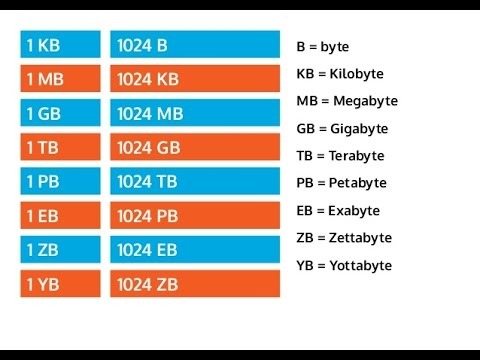
\includegraphics[width=1\textwidth]{figures/Bytes.JPG}}
\caption{gambar Bytes.}
\label{Bytes.JPG}
\end{figure}

\subsection {Cara Mengkonversi}
\subsubsection {A.	Cara Mengkonversi dari Kilo Byte menjadi Mega Byte, Giga Byte dan Tera Byte}

1.	Kilo Byte menjadi Mega Byte
Jika kita memiliki 1000 Kb maka akan menjadi 1 Mb. Karena rumusnya adalah :
Kb : 1000 = Mb
Contoh soal :
Dezha memiliki suatu hardisk berukuran 200000 Kb, Bila Dezha Mengkonversikannya ke dalam Mega Byte maka menghitungnya dengan cara :
200000 Kb : 1000 = 200 Mb
Yang berarti hardisk deza berukuran 200 Mb

2. Megabyte menjadi Kilobyte
jika kita memiliki 1 MB maka akan menjadi 1000Kb maka rumusnya adalah :
Mb x 1000 = Kb
contoh soal :
apabila ilham memiliki suatu file Ms.Word dengan ukuran 4 MB dan dia ingin mengonversikannya ke dalam Kb maka menggunakan rumus: 
4 x 1000 Kb = 4000 Kb
berarti file yang dimiliki oleh ilham adalah berukuran sebesar 4000 Kb

3. Kilobyte menjadi Megabite
Jika kita memiliki file dengan ukuran 1000 Kb dan ingin dikonversikan ke Gb maka rumusnya adalah :
Kylobite : 1000 = Megabyte / 1000
Contoh soal :
Apabila Wahyu memiliki sebuah file dengan ukuran 2.000.000 kb dan ingin dikonversikan ke dalam bentuk gigabyte maka dilakukan :
2.000.000 : 1000 = 2000/1000
=2 Gb
berarti file yang dimiliki wahyu sebesar 2gb
Jadi dapat disimpulan sebelum mengoversikan ke giga harus kita mengkonversi ke mega terlebih dahulu.

4.	Gigabyte menjadi Kilobyte
Jika kita memiliki 1 Gb maka akan menjadi 1000 Mb dengan rumus :
Gb x 1000 = Mb x 1000
= Kb
Contoh : 
Apabila Dudung memiliki sebuah hardisk dengan ukuran kapasitas 20 Gb dan dia ingin mengkonversi kapasitas tersebut ke dalam kb maka di berikan rumus :
20 gb x 1000 = 20000 x 1000
= 200.000.000 kb
Maka kapasitas hardisk dudung sebesar 200.000.000 kb

5.	Kylobyte menjadi Terabyte 
Tom berkata jika ukuran Hardisknya memiliki kapasitas sebanyak 20000000000 Kb dan Mark ingin tahu bahwa bagaimana ukuran hardisk tersebut dalam satuan Terabyte, Maka cara menghitungnya adalah sebagai berikut :
20000000000 Kb : 1000 = 20000000 Mb : 1000 = 2000 Gb : 1000 = 20 TB

6.	Terabyte ke Kilobyte (TB ke Kb)
Jika kita memiliki 1 Tb = 1000 Gb maka jika dikonversi ke kylobyte maka rumusnya sebagai berikut :
Tb x 1000 = Gb x 1000 = Kb
Contoh soal:
Apabila ceu edoh memiliki sebuah hardisk dengan kapasitas 20 Tb dan ingin mengonversikan dalam satuan kylobyte maka cara menghitungnya adalah :
20 Tb x 1000 = 2000 Gb x 1000 
=20.000.000 Mb x 1000 = 2000.000.000
Maka kapasitas hardisk Ceu Edoh adalah 2000.000.000 kb

gambar untuk mengkonversikan gb ke mb \ref{converter.PNG}

\begin{figure}[ht]
\centerline{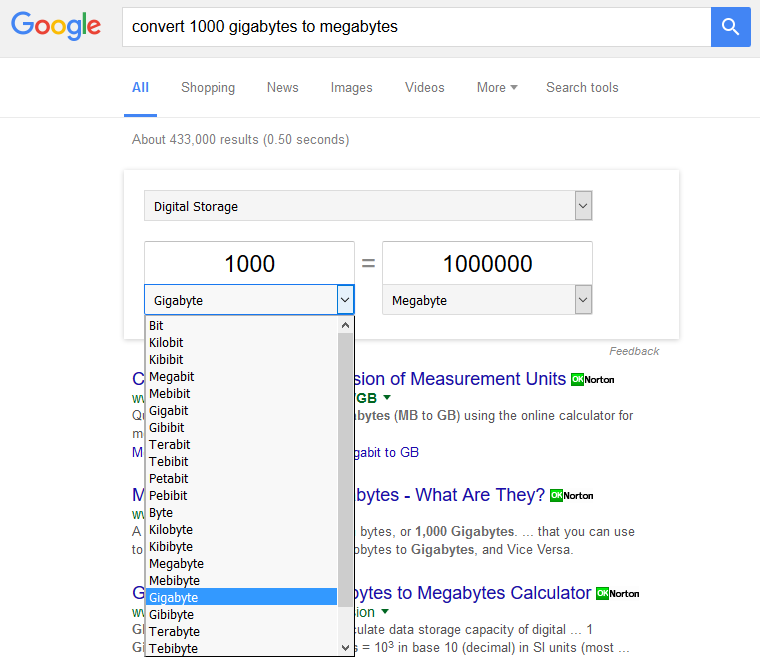
\includegraphics[width=1\textwidth]{figures/converter.png}}
\caption{gambar converter}
\label{converter}
\end{figure}

7.	Megabyte ke Gygabyte (Mb ke Gb)
	Rumus untuk mengkonversi Mb ke Gb adalah (Mb : 1000=Gb)
	Contoh: 
	Tomi ingin mengatakan bahwa flashdisk nya memiliki kapasitas 2000 Mb, maka bila dikonversi  ke dalam Gigabyte adalah 2000 Mb : 1000 : 2 Gb 

8.	Megabyte menjadi Kilobyte
Jika kita memiliki 1 Mb maka akan menjadi 1000 Kb maka rumusnya yaitu :
Mb x 1000 = Kb
Contoh soal :
Apabila Ilham memiliki suatu file Ms. Word dengan ukuran 4 Mb dan dia ingin mengkonversikannya ke dalam Kb maka menggunakan rumus :
4 x 1000 Kb = 4000 Kb
Berarti file milik ilham memiliki berukuran 4000 kb

9.	Megabyte ke Terabyte (Mb ke Tb)
Rumus untuk menghitungnya adalah ( Mb : 1000 = Gb : 1000 = Tb )
Contoh :
Bila Alex Rins mempunyai sebuah folder musik dengan ukuran 2500000 Mb, maka digunakan rumus : 2500000 Mb : 100 = 2500 Gb : 1000 = 2,5 Tb.
artinya alex Rins memiliki folder dengan besar 2,5 Tb.

\subsubsection {B.	Konversi dari Gigabyte ke Terabyte (Gb ke Tb)}

1.	Megabyte ke Gigabyte (Mb ke Gb)
Rumus untuk mengkonversi Mb Ke Gb adalah (Mb : 1000 = Gb)
Contoh :
Tom ingin mengatakan bahwa flasdisknya memiliki kapasitas 2000 Mb, Maka bila dikonversi ke dalam Gigabyte adalah 2000 Mb : 1000 : 2 Gb

2.	Gigabyte ke Megabyte (Gb ke Mb)
Rumus untuk menghitungnya adalah ( Gb x 1000 = Mb )
Contoh :
Jika Iannone memiliki hardisk dengan kapasitas 250 Gb,maka itu artinya adalah Iannone memiliki hardisk 250000 Mb karena 250 x 1000 = 250000 Mb.

C. Konversi dari Gigabyte ke Terabyte (gb ke tb)
1. Terabyte ke Gigabyte (Tb ke Gb)
Rumus untuk menghitung konversi Tb ke Gb adalah ( Tb x 1000 = Gb )
Contoh:
Apabila Jhonatan mengatakan jika dia baru saja menemukan sebuah hardisk dengan kapasitas 20 Tb, dan ingin mengonversikannya ke dalam satuan gigabyte maka jhonatan akan menghitungnya dengan cara sebagai berikut :
20 x 1000 = 20000 Gb.
jadi dapat kita simpulkan bahwa  hardisk yang ditemukan oleh jhonatan berkapasitas sebesar 20000 Gb.

2.	Gigabyte ke Terabyte (Gb keTb)
Rumus untuk menghitung konversi Gb ke Tb  adalah sebagai berikut :
 Gb : 1000 = Tb
Contoh soal :
Jika Valentino Rossi mengatakan bahwa hardisknya memiliki kapasitas 10000 Gb, dan dia ingin mengonversikannya ke dalam satuan terabyte maka ia akan menggunakan rumus :
10000 Gb : 1000 = 10 Tb.
Maka hardisk yang dimiliki valentine berkapasitas sebesar 10 Tb

\subsubsection {D. Mengkonversikan dari satuan Terabyte ke Petabyte}

1.	Dari satuan Tb ke Pb
Rumus untuk mengkonversikan satuan Tb ke Pb adalah sebagai berikut :
Tb : 1000 = Pb
Contoh soal :
Apabila analisa akan mendownload beberapa film yang jika digabungkan memiliki kapasitas 20 Tb akan tetapi ia ingin mengkonversikan ke dalam Petabyte maka 
20 : 1000 = 0.02 Pb
Maka file gabungan film yang dimiliki oleh analisa sebesar 0.02 petabyte
2. Dari satuan Pb ke Tb
Rumus yang digunakan untuk mengkonversika satuan dari Pb ke Tb adalah sebagai berikut :
Pb x 1000 = Tb
Contoh soal :
Jika seorang pejalan kaki menemukan sebuah hardisk berisi kumpulan file yang berkapasitas 5 petabite dan ia ingin mengonversikan hardisk tersebut ke dalam satuan terabite maka akan di gunakan rumus :
5 x 1000 = 5000 Tb
Maka dapat disimpulkan bahwa hardisk yang ditemukan pejalan tersebut berukuran 5000 tb

\subsubsection {E. konversi dari satuan Exabite ke Petabyte atau sebaliknya}

1. Dari satuan Exabyte ke petabyte
Rumus yang akan digunakan dalam satuan ini yaitu :
Eb x 1000 = Pb
Maka apabila kalian memiliki 1 exabyte berarti kalian memiliki kapasitas setara dengan 1 petabyte.
Contoh soal :
Pada suatu hari Eminem menemui sahabatnya, dan sahabatnya tersebut memberikan sebuat laptop dengan kapasitas penyimpanan 15 exabyte kemudian ia ingin mengonversikannya menjadi terabyte maka :
15 Eb x 1000 = 15000 Pb maka laptop tersebut berkapasitas 15000 petabyte.
2.Konversi dari Petabyte ke Exabyte
Rumus yang akan digunakan dalam satuan ini yaitu :
Pb : 1000 = Eb
Maka apabila kalian memiliki 1 Pb berarti kalian memiliki kapasitas setara dengan 0.001 exabyte.
Contoh soal :
Pada suatu hari rosidah membeli computer dengan kapasitas penyimpanan sebesar 5 pb dan seseorang beratanya berapa Eb kah computer yang dimiliki rosidah maka rosidah akan menggunakan rumus sebagai berikut :
5 : 1000 = 0.005 exabyte
Maka rosidah dapat menjawab bahwa komputernya berkapasitas 0.005 pb.

\subsubsection {F. Konversi dari satuan Exabyte ke Zettabyte ataupun sebaliknya}
1. Dari satuan Exabyte ke Zettabyte
Pada koversi Eb menuju Zb dapat digunakan rumus seperti berikut :
Eb : 1000 = Zb
maka dapat kita gunakan simpulkan bahwa 1000 exabyte setara dengan 1 zettabyte.
contoh soal :
jika Irsyad memilik sekumpulan alat penyimpanan berukuran 20 exabyte dan ingin memperkecil jumlah byte didalamnya maka apa yang harus ia akan menggunakan satuan Zettabyte yang dirumuskan
20 : 1000 = 0.02 Zettabyte
maka kumpulan alat penyimpanan Irsyad berkapasitas 0.02 Zettabyte
2.dari satuan Zettabyte ke exabyte
Pada konversi ini menggunakan kebalikan dari Eb ke Zb yang dirumuskan dengan :
Zb x 1000 = Eb
maka mari kita lihat contoh soal berikut ini :
Apabila Sumiati memiliki sesuatu alat penyimpanan berkapasitas 0,013 Zettabyte maka berapa Exabyte alat penyimpanan sumiati, maka akan digunakan rumus perhitungan seperti
0,013 x 1000 = 13 Exabyte
Berarti alat penyimpanan yang sumiati miliki berkapasitas sebesar 13 exabyte.

Tetapi dalam kecepatan transfer data dalam telekomunikasi atau dalam sebuah jaringan biasanya menggunakan istilah "bit per detik" atau
bit per secon (bps), dalam satuan yang lebih modern digunakan satuan kilo bit per second (kbps), dan diatasnya lagi ada megabit per second (Mbps)
contohnya adalah jika kita memakai jaringan akan ada keterangan 56 Kbps atau misalnya 10 Mbps. Dan kecepatan transfer data didalam komputer hanya bisa mencapai satuan ukuran yang lebih besar, yaitu megabyte (Mb). Kabel yang digunakan dalam jaringan komputer yang suka di pakai disetiap kantor-kantor  contohnya, dapat mengirim dan menerima data sampai 100 Mb/s atau sama dengan seratus juta byte setiap detiknya. Jika kita melakukan perhitungan kembal,bahwa kecepatan transfer setinggi itu (100 Mb/s) sama dengan kecepatan 11,9 MB perdetik.

\subsubsection {G. Konversi satuan bit lainnya}
Konversi satuan kapasitas byte diatas Zetta byte masih ada pula Yotta byte, Bronto Byte dan, Geo Byte yang mungkin masih ada banyak satuan lainnya yang lebih besar lagi untuk menghitung jumlah kapasitas pada satuan tersebut yaitu apabila naik menuju pada satuan yang lebih kecil maka akan dikalikan dengan 1000 sehingga akan menjadikan angka-angka yang muncul semakin besar dan bertambah. 
Apabila ingin mengkonversi ke satuan yang lebih besar maka akan dibagi dengan 1000 sehingga angka yang akan muncul semakin kecil dan ringkas serta membuat kita mudah untuk mengingatnya apabila dibutuhkan.
\ref{ukuran.PNG}
contoh gambar

\begin{figure}[ht]
\centerline{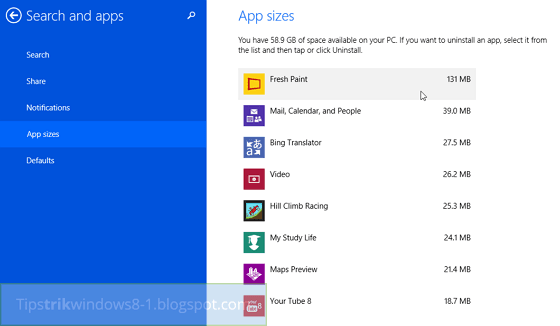
\includegraphics[width=1\textwidth]{figures/ukuran.png}}
\caption{gambar ukuran}
\label{ukuran}
\end{figure}

\section {KESIMPULAN}
Kesimpulan yang dapat kita ambil dari makalah konversi mengenai Bytes ialah sebagai berikut :
1.	Apabila kita ingin mengkonversi dari satuan terkecil menuju terbesar maka menghitungnya dengan cara “:” membagi.
2.	Sedangkan jika kita ingin mengkonversi dari satuan terbesar menuju terkecil maka kita bisa menghitungnya dengan cara “x” mengkali.
3.	Dapat disimpulkan bahwa setiap satuan yang lebih besar akan mendapatkan kenaikan sebanyak 1000 kali dan setiap satuan yang lebih kecil akan mengalami pembagian sebanyak 1000 kali pula.
4.	Dengan adanya konversi ini kita tidak perlu menggunakan angka yang berjumlah ribuan, jutaan, hingga milyaran sekalipun menggunakan angka yang lebih kecil dengan satuan yang besar.
5.	Melalui konversi ini kita dapat menghitung berbagai jumlah kapasitas dari perangkat-perangkat penyimpanan yang kita miliki, oleh karena itu mempelajari konversi ini sangatlah penting dan bermanfaat bagi kehidupan kita. \cite{jungwirth2002information}